The \sh settings are divided into two types. There are global preferences and settings for a specific view. All settings are stored in the database. Therefore your settings travel with your profile.

\begin{figure}[!htb]
   \centering
   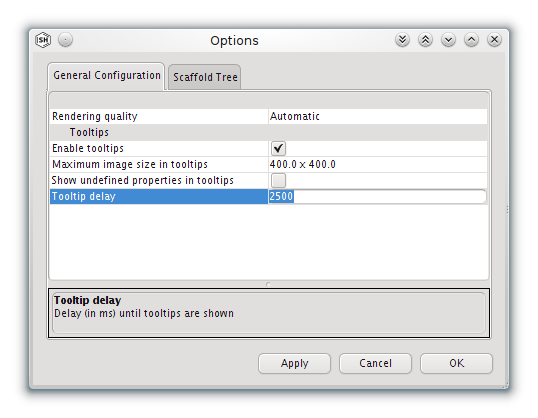
\includegraphics[width=0.5\textwidth]{images/sh_preferences_dialog_generalconfiguration.png}
   \caption{Preferences Dialog}
   \label{fig:generalconfiguration}
\end{figure}
\paragraph{Preferences}
The global preferences are accessible via \texttt{Session $\rightarrow$ Preferences} in the menu bar. The Dialog \figref{fig:generalconfiguration} has a \texttt{General Configuration} tab with settings that will apply to all views and the main window. The options are self explaining. If you select an option by clicking on it you get a more detailed description in the label below. 

There are also tabs for types of views. For example you can find general options for the \stview. These settings will apply to all views of one type that are open (e.g. all \stviews). Currently only the \stview uses this global settings, but in future there may be also other views available here. 

\begin{figure}[!htb]
   \centering
   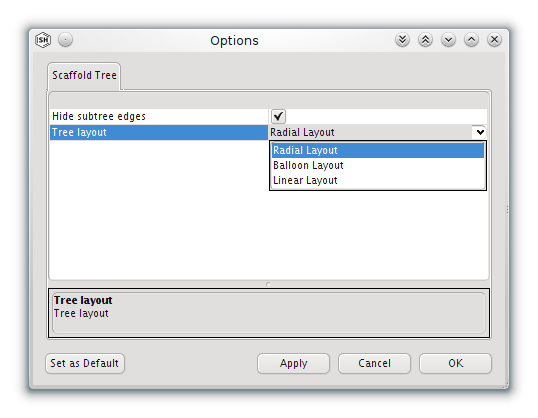
\includegraphics[width=0.5\textwidth]{images/sh_configure_view_dialog_scaffoldtree.png}
   \caption{Configure View Dialog}
   \label{fig:configure_view}
\end{figure}
\paragraph{Configure View}
The preferences for one specific view are accessible over \texttt{Session $\rightarrow$ Configure View}. The dialog \figref{fig:configure_view} has the same layout as the global preferences. It shows one tab for each open view. If you have two open \stviews you will find two tabs here. The name of the tabs matches the name of the view tabs in the main window. Renaming the views can thereby significantly improve the assignment between preferences tabs and the corresponding view (see \secref{sec:scaffoldhunter:viewmanagement:renaming}). Some options may also be available directly over the menu bar or \tbar (for further details see \secref{sec:scaffoldhunter:views}).